\section{Methodology}

Providing a macroscopic view on where traffic originates from, and in what quantity, can be achieved by simply binning packets into flows and accumulating byte counts over geographical or topological locations. 
Uncovering application layer characteristics (i.e. \textit{how} traffic is sent) is a more complex problem that requires additional methods to reverse engineer transport behaviour.
The aim of this section is to describe a process which distinguishes those flows which have their throughput limited by mechanisms other than the usual \ac{TCP} response to loss and delay.
Each flow can be characterized as being either application paced, in which the sending application is limiting the data provided, host limited, whereby local constraints at either end host cap throughput, or receiver shaped, in which an artificial constraint is imposed by either a middlebox or receiver.

The classification proceeds in stages. 
Before classification, it is necessary to reconstruct the RTT of the flow if the flow is not bidirectional.  
This is achieved in section \ref{subsection:malawi:PeriodicEnhancement}. 
Because the sender's TCP state machine cannot be directly observed it is necessary then to estimate the size of the congestion window by observing the number of unacknowledged bytes in flight (\textit{flight size}).
This reconstruction is described in section \ref{subsection:malawi:flightAggregation} and provides the basis for flow classification. 
Flows are then checked in turn to see if they are application paced, host limited or receiver shaped and classified as belonging to the first of these classes for which they fulfill the necessary conditions.
Flows in none of these classes are either limited only by the network (delay or loss conditions) or are insufficiently large to trigger any further constraints.

\subsection{\acs{RTT} Estimation}
\label{subsection:malawi:PeriodicEnhancement}

Building on prior work presented in section \ref{section:malawi:related}, this section proposes an algorithm that scalably recovers the RTT from one-directional traffic traces. 
% XXX: below implies microflights were used, but these aren't described (remove as appropriate)
Although \ac{RTT} estimation is a difficult problem, simplifying assumptions can be made.
For the \acs{MAWI} dataset most \acp{RTT} are relatively large, with the closest neighbouring country, South Korea, roughly 40ms away.
By only processing bidirectional traffic from Japan, the expected \ac{RTT} range can be reduced for all other traffic.
The recovery mechanism then enhances the natural periodicity of traces and scalably constructs flights associated with specific application and protocol behaviour.
In the following the mechanisms required by these two goals are described. 
%
% Why does this work?
%
In normal operation, many \ac{TCP} operations involve request-response cycles between two endpoints in which the \ac{RTT} $T$ provides a natural \emph{clock}.
Hence, the most natural way to estimate \ac{RTT} from \ac{TCP} traces is to correlate requests and responses exchanged in both directions. 
If only one direction of data is observed however, $T$ cannot be directly observed. 
Instead, it must be estimated from the way in which \ac{TCP} packets cluster in time due to the batching of request-response operations.

The \ac{TCP} \ac{cwnd} determines the number of unacknowledged bytes that a \ac{TCP} flow may maintain at any point in time. 
This can be referred to as \emph{bytes in flight} because they are in transit between the sender $S$ and the receiver $R$; an equivalent definition applies for the number of \emph{packets in flight}. 
Once $S$ has transmitted \ac{cwnd} data bytes, it will refrain from transmitting more until either some bytes are acknowledged by $R$ or \ac{cwnd} is increased by the sender. 
In the absence of losses, neither of these events can happen until a \ac{TCP} \ac{ACK} is received; this immediately reduces the number of unacknowledged bytes, but may also lead to a significant \ac{cwnd} increase (during e.g. \emph{slow start}). 
% XXX: number of unacknowledged bytes reduced, or CWND?
In the presence of losses, however, bytes can be re-sent if a packet is timed out and considered lost; in this case, the number of unacknowledged bytes is reduced.

%
% What is our main contribution, algorithmically speaking?
%
The main difficulty associated with one-sided TCP flow reconstruction is as follows.
Let $t_1, t_2, \ldots$ be a set of times at which packets $p_1, p_2, \ldots$ were observed at $S$ en route to $R$.
Suppose that a packet $p_j$ of size $b$ is observed at time $t_j$.
In addition, suppose that approximately one RTT $T$ later, the sender $S$ receives an ACK $a_j$ from $R$ for the $b$ bytes of $p_j$.
At this point, the TCP stack in $S$ will decrease the number of unacknowledged bytes by $b$, thus opening the possibility for sending additional traffic to $R$.
This can lead to another packet $p_k$ to be transmitted; let this packet be observed at time $t_k$ as it is sent towards $R$.
Assuming that processing delay is insignificant, the RTT experienced by $p_j$ can be approximated as $T \approx t_k - t_j$.
Now consider what happens if packets are only observed in the $S \rightarrow R$ direction.
Under such conditions, it is not possible to ascertain whether $p_k$ was sent explicitly as a result of $S$ receiving the unobserved \ac{ACK} $a_j$, or whether it was sent as a result of an \ac{ACK} $a_i$ associated with a previous packet $p_i$ rather than with $p_j$.
If, however, a packet $p_l$ is eventually observed that did result from the reception of $a_j$, the \ac{RTT} can be estimated as $T \approx t_l - t_j$ with $t_l > t_k$.
Following this same reasoning, approximately one \ac{RTT} later a packet $p_m$ will be observed for which $2T \approx t_m - t_j$; this can potentially continue for as long $S$ has data to send and $R$ continues sending \acp{ACK}.
This is the underlying reason that \ac{RTT}-related periodic regularities arise when considering the timestamps of observed packets \cite{Qian:2009p429}.

The reasoning above is at the heart of the proposed algorithm to improve \ac{RTT} recovery by enhancing packet stream periodicity. 
Assume that a packet $p_j$ is observed at time $t_j$. 
Considering the set $\mathcal{T}_j$ of all values of $\Delta t = t_k - t_j$ for every $k > j$, it is apparent that it will include estimates not only for the \ac{RTT} $T$, but also for all its multiples $2T, 3T, \ldots$ 
If $t_l-t_k \approx T$ and $t_k - t_j \approx T$ then it follows that $t_l - t_j = 2T$, and this value will also be included in $\mathcal{T}_j$. 

By maintaining a set $\mathcal{T}_j$ for every packet $p_j$ observed, at least some of its values will correspond to estimations of multiples of the \ac{RTT}. 
It then follows that by creating a set $\mathcal{T}$ that includes values calculated starting from every packet $p_j$ so that $\mathcal{T} = \cup_j \mathcal{T}_j$, numerous estimates for $2T, 3T, \ldots$ will also be included. 
Hence, the probability density function $H(t)$ of the values in $\mathcal{T}$ should show peaks around multiples of the \ac{RTT} (see Figure \ref{fig:histogram}). 

\begin{figure}
  \centering
  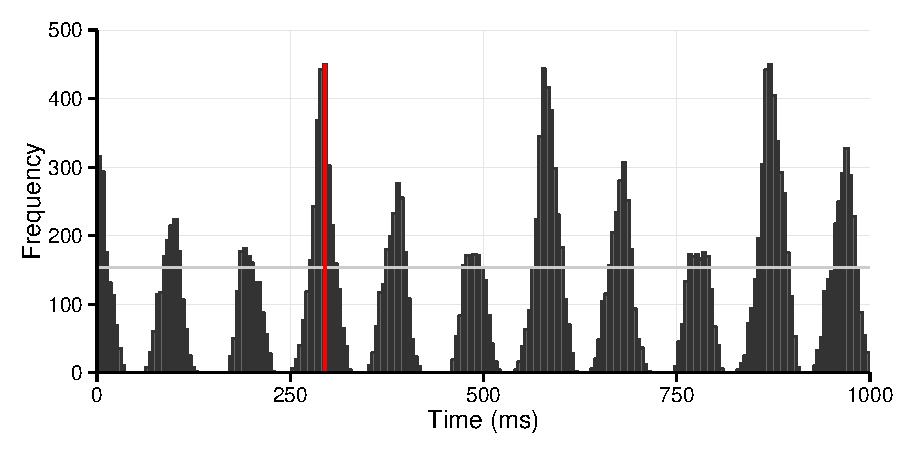
\includegraphics[width=0.8\textwidth]{figures/malawi/rttbin.pdf}
  \caption{$H(t)$ for flow displayed in Figure \ref{fig:hostlimited}. The horizontal line delimits $\overline{H}$ while the highlighted bin denotes the bidirectional RTT estimate.\label{fig:histogram}}
\end{figure}

%
% Explain why did we use FFT
%
The algorithmic recovery of $T$ from $H(t)$ presents additional challenges. 
In particular, $H(t)$ may include a large number of \ac{RTT} multiples, and a peak will be found for all of them. 
Crucially, all these peaks may be of comparable magnitude, complicating the task of selecting a single peak.
Moreover, these peaks need not be very pronounced, with histogram bins in close proximity of the peaks have very similar values as the peak itself. 
As such, taking \ac{RTT} candidates directly from $H(t)$ may result in a large set of similarly-valued bins situated around a peaks at multiples of the \ac{RTT}. 

Three recovery algorithms for $T$ are attempted.
First, as a baseline, the highest peak in $H(t)$ is selected as a candidate for $T$. 
In addition, expanding upon the work of Qian et. al. \cite{Qian:2009p429} a frequency-domain representation of $H(t)$ is used to identify $T$. 
This is done by selecting the highest peak of $|\hat{H}(\omega)|^2$, the \emph{energy spectral density} of $H(t)$ (i.e. the norm squared of the Fourier transform of $H(t)$). 
Finally, a custom utility-based technique that operates directly on $H(t)$ is proposed which achieves superior performance to both of the aforementioned methods.

%\subsubsection{FFT-Based RTT Recovery}
%We extract periodicity information from $H(t)$ by looking at $\hat{H}(\omega)$, the \emph{energy spectral density} of $H(t)$. Formally, $\hat{H}(\omega)$ is defined as the norm squared of the Fourier transform of $H(t)$, so that $\hat{H}(\omega) = |\mathcal{F}(H(t))|^2$. Using $\hat{H}(\omega)$ markedly improves the quality of our RTT estimation because the frequency peak corresponding to the RTT usually accounts for a much larger proportion of the total frequency domain energy than other peaks in $\hat{H}(\omega)$, leading to a much simpler discrimination of the true RTT. However, due to RTT changing during the lifetime of a flow, and also due to the expected noise associated with real-life data sources, $\hat{H}(\omega)$ can also occasionally include large peaks at frequencies unrelated to the RTT. In order to filter these out, we take a set of 10 frequency candidates from $\hat{H}(\omega)$, and use their associated periods as RTT candidates in our flow reconstruction algorithm (see Section \ref{
%subsection:malawi:flightAggregation}). We then select that RTT candidate which exhibits the smallest error, that is, that one which yields closest agreement with observed data.

%
% Algorithmic hacks
%
%To streamline our algorithm for streaming use, we use the following heuristics and approximations. Firstly, we define a range $[T_{\min}, T_{\max}]$ representing the range over which we find the RTT values of interest. Then, for each packet $p_j$, we build a subset $\mathcal{T}_j'$ of $\mathcal{T}_j$ by including all values of $t_j - t_k < T_{\max}$. We then generate $\mathcal{T}' = \cup_j \mathcal{T}_j'$ and approximate $H(t)$ by considering a histogram of the values in $\mathcal{T}'$. As usual, we do this by counting the frequency with which its values are observed in the ranges $[0,\tau)$, $[\tau, 2\tau)$, $[2\tau, 3\tau), \ldots$ where $\tau$ is the time resolution required. 


\subsubsection{Utility-Based RTT Recovery}
\label{sect:utilityBasedRecovery}

This method relies not on the identification of periodicities, but on explicitly matching experimentally found signatures. 
To this end, we consider the peaks of $H(t)$, which are then considered RTT candidates.  
However, trivial discriminators (such as simply selecting the highest peak) are not reliable. 
In this case, it was found experimentally that repeatable peaks and troughs also occur at multiples and sub-multiples of $T$, with the most important ones being $\frac{T}{3}$, $\frac{T}{2}$, $T$ and $2T$. 
We design this detection algorithm around the idea that a given pattern of peaks and troughs can identify $T$.

If we define $\overline{H}$ as the mean height of $H(t)$, we can define a per-peak utility function $p(t)$ so that 
\begin{equation*}
p(t) = 1.0 - \exp\left(-2.0 \left(\frac{H(t)}{\overline{H}}\right)\right) \mbox{.}
\end{equation*}
This function has several advantageous properties: it is 0 if $H(t)$ is zero, 1
if $H(t)$ is infinite, and $0.5$ if $H(t) = \overline{H}$.  In other
words it is a measure of the \emph{peakiness} of the data, with $p=1$ identifying
an infinitely high peak, $p=0$ identifying an empty histogram bin (trough), and $p=\frac{1}{2}$ 
implying that $H(t)$ is of exactly average height at that point. We can then score each candidate using the following utility function:
$$
P(t) = 1.5 p(t) + p(2t) - p\left(\frac{t}{2}\right) - p\left(\frac{t}{3}\right).
$$
That is, the candidate RTT $t$ scores highly if it is itself a peak, if it has a peak
at a multiple $2t$, and if it also manifests troughs at submultiples $\frac{T}{2}$ and $\frac{T}{3}$.
The factor of 1.5 was added after observations
showed that the peak at $T$ was the most important factor in determining
whether a candidate was the true RTT. Similarly, additional multiples and submultiples 
were excluded as they showed very limited discriminating power experimentally.

\begin{figure}
  \centering
  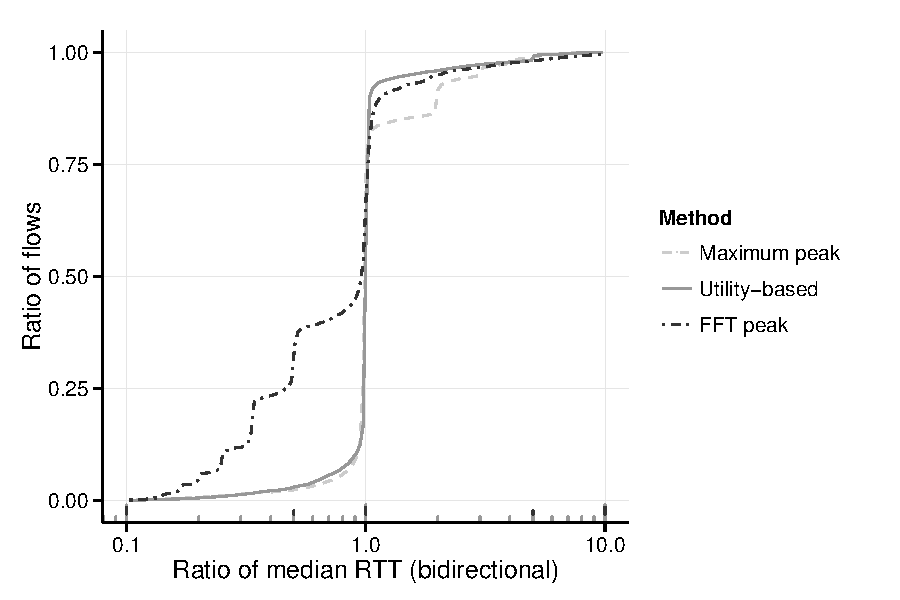
\includegraphics[width=0.8\textwidth]{figures/malawi/rttcomp.pdf}
  \caption{Accuracy of RTT estimator when compared to the median value of bidirectional estimate.}
\end{figure}

\subsubsection{Comparing RTT Recovery Algorithms}
\label{sect:comparingRecoveryAlgos}
As described in Section \ref{subsection:malawi:PeriodicEnhancement}, $H(t)$ is calculated in such a way that RTT periodicity is amplified. 
This means that FFT-based techniques could potentially perform better on $H(t)$ than on the packet stream with no pre-processing. 
However, this is complicated not only because $H(t)$ contains periodicities at multiples of $T$, but also discontinuities that generate harmonics at frequency multiples of the RTT fundamental. 
Hence, although the FFT $|\hat{H}(\omega)|$ of $H(t)$ is much cleaner than that of the packet interarrival time series on its own, its maximum peak rarely coincides exactly with the RTT clock (this corroborates reports by Qian et al \cite{Qian:2009p429}). 
Thus, applying the FFT leads to another \emph{peak detection problem} in which the RTT fundamental needs to be extricated from its harmonics and sub-harmonics. 
The trivial solution to this problem, the application of a bandpass filter around the RTT frequency, is of course unfeasible because the bandwidth and 
centring of such a filter depend on the RTT which is itself unknown.
The utility-based algorithm described in Section \ref{sect:utilityBasedRecovery} can hence be applied in either the time domain or the frequency domain; we chose to do it on the former on the interest of expediency and lower computational cost.

\newcommand{\RTTHeader}{Below & Above}
\newcommand{\SmallFlowName}{\textless 10MB}
\newcommand{\LargeFlowName}{\textgreater 10MB} 
\begin{table}
\footnotesize
\centering
\begin{tabular}{ p{1.5cm} p{1.2cm} p{0cm} p{.6cm}p{.6cm} p{0cm} p{.6cm}p{.6cm}}
& & & \multicolumn{2}{c}{Peak} & & \multicolumn{2}{c}{Utility-based} \\
\cline{4-5} \cline{7-8}
& Flow size & & \RTTHeader & & \RTTHeader \\
\cline{4-5} \cline{7-8} 
\multirow{2}{*}{Receiver side}  & \SmallFlowName && 4.31 & 9.13 && 4.58 & 6.35
\\ 
                                & \LargeFlowName && 6.72 & 6.43 & 4.97 & 5.33
\\
\multirow{2}{*}{Sender side}    & \SmallFlowName && 2.94 & 8.37 && 3.29 & 4.80
\\
                                & \LargeFlowName && 6.41 & 9.06 & 5.40 & 11.06
\\
\end{tabular}
\caption{\label{table:rttRecovery}Performance of RTT recovery algorithms}
\vspace{-3mm}
\end{table}

The performance of the analysed RTT recovery mechanisms is presented in Table \ref{table:rttRecovery}, that shows the percentage of total flows below and above the RTT range given by the bidirectional estimates.
We separate things for \emph{inbound} traffic (where we are positioned at the receiver side) and \emph{outbound} traffic (where we are positioned at the sender side). The utility-based algorithm is particularly useful to address RTT underestimation for flows over 10MB in size, which is our main objective since precisely that kind of estimation error would interfere with our ability to correctly decouple application behaviour from RTT-scale dynamics.


%For the most part, the utility based method improves on underestimation, which is our main objective since that would interfere with our flight reconstruction (i.e. generate lots of gaps).
%The exception (kind of) is traffic from the sender side, which in our training set (one week per year), had quite a lot of host limited traffic (paced out, no signal to recover).
%In this case, not a problem, since if the flow is long enough multiples of the RTT will still reveal host limitation, but will give us a smaller window..


\subsection{Flow Classification}
\label{subsection:malawi:flightAggregation}

One fundamental precondition to decouple the influence that network loss, host configuration and TCP behaviour has on the throughput experienced by a flow is the reconstruction of the congestion window behaviour of TCP flows on the basis of observed data. 
Unfortunately, the congestion window value is internal to the sender's TCP state machine and may not manifest itself in the absence of sufficient data from the application layer. 
A more easily observed quantity which serves as a reasonable proxy for the congestion window is the number of unacknowledged bytes in flight, henceforth referred to as the \textit{flight size}, which can be derived given an accurate estimate of the end-to-end delay.
The evolution of both flight size and RTT can in turn be used to ascertain to what extent throughput is regulated by limitations imposed at different layers of the networking stack.

% definitions
Given a candidate RTT, we can aggregate a stream of packets with arrival times $t_1, t_2, \ldots$ into a stream of \emph{flights}. 
Intuitively, a flight is a clustered subset of a TCP flow which exhibits its own temporal coherence; alternatively, it can be though of as a series of consecutive packets that were (roughly) generated by the sender as a response to the same protocol operation. 
A flight $f_i$ that begins
with the $j$th packet and ends with the $k$th is defined to have a \emph{total flight time} $\tau_i = t_{k+1} - t_j$. 
The algorithmic selection of initial and final packets in such a way that the resulting flights are indicative of TCP behaviour remains an open problem. 
Since we assume that the RTT provides a natural time frame for the operations of TCP, in the algorithm presented in this work, given an initial packet $\pi_j$ and an RTT estimate $T$, the $k$th (and final) packet is selected to minimise \emph{the flight time error} $e_i = |T - \tau_i|$. 
This mechanism follows closely the methodology described in \cite{Zhang:2002p85}, with the exception that we do not attempt to define flights as being both adjacent and disjoint; rather, we decompose flows into a stream of potentially overlapping flights. 
This helps the algorithm mitigate the deleterious effects of small deviations in the estimated RTT, which alters the properties of each flight. 
Furthermore, since the flight size is continuous in time, it makes little sense to restrict ourselves to a single sample per round trip time.

Having obtained flight information from each flow, we next consider what is the predominant factor that affects its throughput. 
Within the context of TCP, we classify flows as being artificially constrained by three distinct processes: \emph{application pacing}, \emph{host limited} and \emph{receiver shaping}.

\begin{figure}
\centering
  \centering
  \begin{subfigure}{1.0\linewidth}
    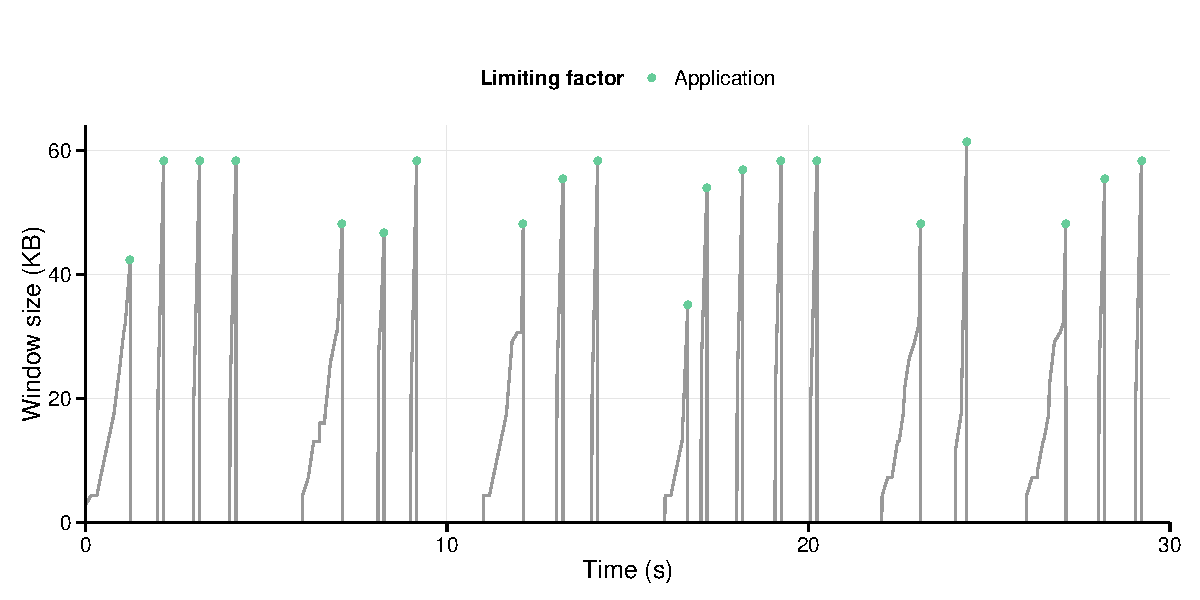
\includegraphics[width=1.0\textwidth]{figures/malawi/youtube.pdf}
    \caption{Application paced. \label{fig:youtube}}
  \end{subfigure}\\
  \begin{subfigure}{1.0\linewidth}
    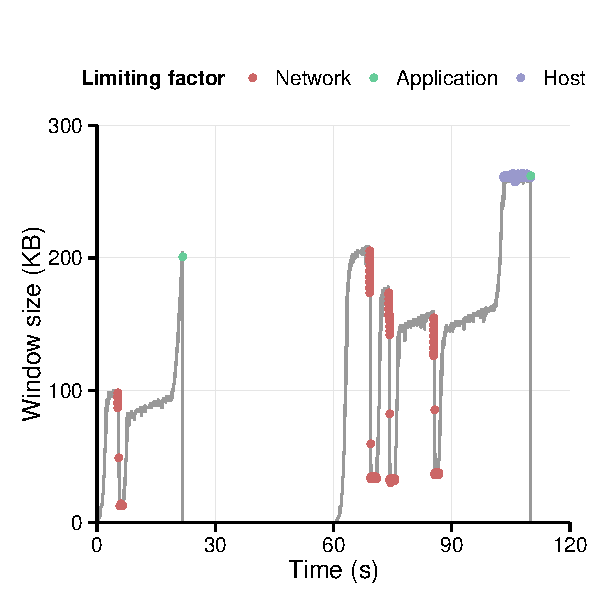
\includegraphics[width=1.0\textwidth]{figures/malawi/hostflow.pdf}
    \caption{Partially host limited. \label{fig:hostlimited}}
  \end{subfigure}\\
  \begin{subfigure}{1.0\linewidth}
    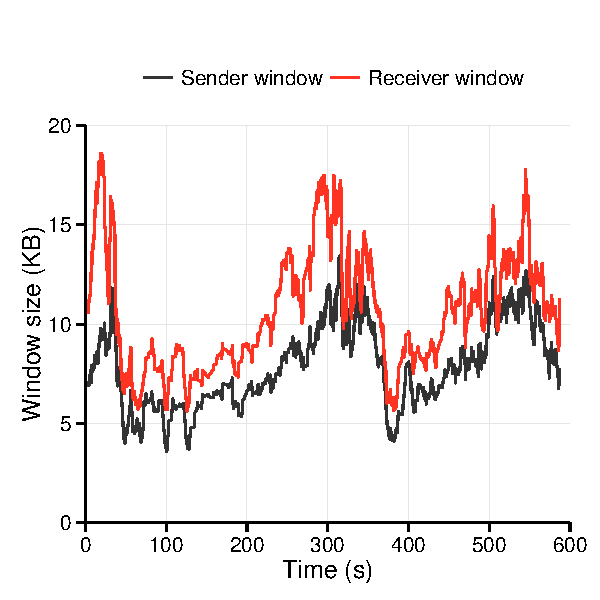
\includegraphics[width=1.0\textwidth]{figures/malawi/awnd.pdf}
    \caption{Receiver shaped. \label{fig:awnd}}
  \end{subfigure}
  \caption{Flight size over time for flows affected by different artificial constraints. \label{fig:kindsOfFlowEffect}}
\end{figure}


\subsubsection{Application Paced Flows}
\label{sssec:app}

A flow whose throughput decreases because it has no outstanding data to send is temporarily limited by the application. 
Flights can be identified as being \emph{application limited} if terminated with a packet smaller than the maximum segment size (MSS) and followed by an inter-arrival time greater than the RTT, as consistent with \cite{Zhang:2002p85}. 
The underlying reason for this defintion is that most TCP implementations will wait some time for subsequent bytes to be written to the socket if the next packet to be sent is smaller than the MSS, unless the TCP\_NODELAY option is set \cite{nagle1984rfc}.

A flow with \emph{application limited} flights however is not necessarily \emph{application paced}. In practice, all flows for which the final packet is observed contain at least one such flight.
For the purposes of our work, we are focused on identifying cases in which throughput is predominantly determined by application behaviour.
One such example is illustrated in figure \ref{fig:youtube}, in which a stream is delivered by periodically writing blocks to the sending socket.
The resulting network-level behaviour is distinct from traditional congestion control: short bursts are interspersed with protracted silence.
Application limited flights, which terminate on non-MSS packets, are highlighted at the end of each burst.

This behaviour is in stark contrast to that exhibited in figure \ref{fig:hostlimited}, where distinct transfers are multiplexed on top of a single transport association over time.
From the perspective of the network, there is little to distinguish the behaviour of such traffic from independent TCP flows.
Application paced connections such as Youtube traffic however exhibit a degree of regularity which can potentially be exploited by the network in predicting demand or smoothing bursts.

In order to identify such recurring behaviour, we identify flows as being \emph{application paced} if the period between bursts terminated by \emph{application limited flights} is consistently under 10 seconds and the standard deviation of the intermediate pauses is under one second.
This definition in particular purposely ignores flows which exhibit long silence periods due to user interaction, and follows closely the behaviour historically associated to Youtube streaming in particular.

\subsubsection{Host Limited Flows}
\label{sssec:host}

Given sufficient bandwidth and traffic to send, a flow may encounter local constraints at either end-host which cap its throughput. 
For instance, the buffer space allocated on both the sender and receiver side is often pre-configured, and it is common practice to tune these values down on popular servers and managed infrastructure in a bid to conserve memory or bandwidth.
A receiver is also limited in the window size it can announce to the remote sender; if the windowscale option \cite{jacobson1992tcp} is not negotiated during the TCP handshake, the advertised window cannot exceed 64KB.

In both cases, a local decision by either host can determine the upper bound of the flow rate.
These \emph{host limited} cases are characterised by a constant window size over time.
The methodology described for flight aggregation at the beginning of this section typically generates a large number of flights, representing many likely combinations given a base RTT estimate.
In order to identify the flat-lined behaviour of a host limited flow, we first filter the flight stream to remove some of the uncertainty derived from small fluctuations in the RTT.
We then select the maximum flight size observed for each RTT interval, and declare a sequence of flights to be host limited if the same maximum was observed over six consecutive RTTs (this is twice the period suggested in \cite{Zhang:2002p85}).
In practice, increasing the period over which the maximum window size is tracked allows us to more accurately discern between host limited behaviour and more conservative bandwidth probing, such as that performed during the convex phase of TCP CUBIC \cite{Ha:2008p471}.

A flow may be host limited for only brief periods of its lifetime, as illustrated in figure \ref{fig:hostlimited}.
To filter out such cases where host limitations are not the predominant factor in defining flow throughput, we further enforce that in addition to host-limited flights, the average window size must over a flow lifetime should be within 10\% of the inferred host limit, which is not the case in figure \ref{fig:hostlimited}.

In practice, flows can exhibit both application pacing and host limitations, with bursts being sent at a capped window size followed by application pauses.
In such cases, a flow will still be classified as being \emph{application paced} if it meets the requirements set out in the previous section, as doing so provides evidence that it controls throughput in spite of the degraded performance provided further down the stack. 
This line of reasoning applies equally to the occurrence of sporadic loss; so long as block delivery is ensured within the timeframe dictated by the application, it remains in control.

\subsubsection{Receiver Shaped Flows}
\label{sssec:rec}

A flow which is neither \emph{application paced} or \emph{host limited} can still be artificially constrained by flow control (rather than by congestion control).
Traditionally, in TCP the sender is responsible for regulating throughput. 
However, the receiver can also shape throughput by manipulating the \emph{advertised window} announced on every acknowledgement.
Such receiver-window auto-tuning has been available on Windows operating systems since Vista \cite{vistaReceiveWindow}, and can also be leveraged by middleboxes in order to throttle inbound traffic \cite{appEx}.

In order to evaluate the potential impact of such behaviour, we further propose a heuristic to identify receiver-shaped traffic.
For flows in which both directions of traffic are observed it is possible to correlate the evolution of the advertised window with the size of reconstructed flights.
Figure \ref{fig:awnd} displays an example of a receiver-shaped connection, in this case throttled by an intermediate middlebox.
Since the advertised window may be fluctuating, it is not always obvious which of the many updates were effectively applied by the sender as successive values supersede each other.
An example of a reconstructed flow which is subjected to receiver shaping is displayed in Figure \ref{fig:awnd}.

For flows in which both directions are observed, it is possible to classify flights as being receiver-shaped if there is a statistically significant correlation between the advertised window size and the maximum flight size observed.
Harnessing the stream filtering used in detecting host limited behaviour, we perform such analysis over a sliding window of 10 RTT intervals.
A flight is flagged as being receiver shaped if the correlation between receiver window and flight size is statistically significant; a flow is considered to be predominantly receiver shaped if over half of its flights are flagged as such.
We do not perform this covariance analysis on flights which contain out-of-order or retransmitted packets. 
In these cases, both the receiver and sender window sizes are correlated \emph{by definition}. 
In the former case, the receiver buffer will temporarily fill expecting the next packet in sequence, in the latter case, TCP will reduce its window.

Given that receiver shaping classification requires correlating information in both directions of a TCP connection, it will come as no surprise that the absence of the reverse path can introduce false positives into our measurements. 
This happens because any given flow might be receiver shaped in such a manner that the heuristic erroneously attributes its behaviour to host limitations. 
In the absence of additional evidence, this misclassification is difficult to detect explicitly. 
Instead, we calculate the ratio of receiver shaped flows which would have been incorrectly identified if the reverse path were not observed. 
This error rate can then be used to evaluate the accuracy of classifier results.
